% VDE Template for EUSAR Papers
% Provided by Barbara Lang und Siegmar Lampe
% University of Bremen, January 2002
% English version by Jens Fischer
% German Aerospace Center (DLR), December 2005
% Additional modifications by Matthias Wei{\ss}
% FGAN, January 2009

%-----------------------------------------------------------------------------
% Type of publication
\documentclass[a4paper,10pt]{article}
%-----------------------------------------------------------------------------
% Other packets: Most packets may be downloaded from www.dante.de and
% "tcilatex.tex" can be found at (December 2005):
% http://www.mackichan.com/techtalk/v30/UsingFloat.htm
% Not all packets are necessarily needed:
\usepackage[T1]{fontenc}
\usepackage[latin1]{inputenc}
%\usepackage{ngerman} % in german language if required
\usepackage[nooneline,bf]{caption} % Figure descriptions from left margin
\usepackage{times}
\usepackage{multicol}
\usepackage{amsmath}
\usepackage{amssymb}
\usepackage{graphicx}
\usepackage{epsfig}
% Macros for Scientific Word 3.0 documents saved with the LaTeX filter.
%Copyright (C) 1994-97 TCI Software Research, Inc.
\typeout{TCILATEX Macros for Scientific Word 3.0 <05 August 1998>.}
\typeout{NOTICE:  This macro file is NOT proprietary and may be 
freely copied and distributed.}
%
\makeatletter
%
%%%%%%%%%%%%%%%%%%%%%%
% macros for time
\newcount\@hour\newcount\@minute\chardef\@x10\chardef\@xv60
\def\tcitime{
\def\@time{%
  \@minute\time\@hour\@minute\divide\@hour\@xv
  \ifnum\@hour<\@x 0\fi\the\@hour:%
  \multiply\@hour\@xv\advance\@minute-\@hour
  \ifnum\@minute<\@x 0\fi\the\@minute
  }}%

%%%%%%%%%%%%%%%%%%%%%%
% macro for hyperref
\@ifundefined{hyperref}{\def\hyperref#1#2#3#4{#2\ref{#4}#3}}{}

% macro for external program call
\@ifundefined{qExtProgCall}{\def\qExtProgCall#1#2#3#4#5#6{\relax}}{}
%%%%%%%%%%%%%%%%%%%%%%
%
% macros for graphics
%
\def\FILENAME#1{#1}%
%
\def\QCTOpt[#1]#2{%
  \def\QCTOptB{#1}
  \def\QCTOptA{#2}
}
\def\QCTNOpt#1{%
  \def\QCTOptA{#1}
  \let\QCTOptB\empty
}
\def\Qct{%
  \@ifnextchar[{%
    \QCTOpt}{\QCTNOpt}
}
\def\QCBOpt[#1]#2{%
  \def\QCBOptB{#1}
  \def\QCBOptA{#2}
}
\def\QCBNOpt#1{%
  \def\QCBOptA{#1}
  \let\QCBOptB\empty
}
\def\Qcb{%
  \@ifnextchar[{%
    \QCBOpt}{\QCBNOpt}
}
\def\PrepCapArgs{%
  \ifx\QCBOptA\empty
    \ifx\QCTOptA\empty
      {}%
    \else
      \ifx\QCTOptB\empty
        {\QCTOptA}%
      \else
        [\QCTOptB]{\QCTOptA}%
      \fi
    \fi
  \else
    \ifx\QCBOptA\empty
      {}%
    \else
      \ifx\QCBOptB\empty
        {\QCBOptA}%
      \else
        [\QCBOptB]{\QCBOptA}%
      \fi
    \fi
  \fi
}
\newcount\GRAPHICSTYPE
%\GRAPHICSTYPE 0 is for TurboTeX
%\GRAPHICSTYPE 1 is for DVIWindo (PostScript)
%%%(removed)%\GRAPHICSTYPE 2 is for psfig (PostScript)
\GRAPHICSTYPE=\z@
\def\GRAPHICSPS#1{%
 \ifcase\GRAPHICSTYPE%\GRAPHICSTYPE=0
   \special{ps: #1}%
 \or%\GRAPHICSTYPE=1
   \special{language "PS", include "#1"}%
%%%\or%\GRAPHICSTYPE=2
%%%  #1%
 \fi
}%
%
\def\GRAPHICSHP#1{\special{include #1}}%
%
% \graffile{ body }                                  %#1
%          { contentswidth (scalar)  }               %#2
%          { contentsheight (scalar) }               %#3
%          { vertical shift when in-line (scalar) }  %#4
\def\graffile#1#2#3#4{%
%%% \ifnum\GRAPHICSTYPE=\tw@
%%%  %Following if using psfig
%%%  \@ifundefined{psfig}{\input psfig.tex}{}%
%%%  \psfig{file=#1, height=#3, width=#2}%
%%% \else
  %Following for all others
  % JCS - added BOXTHEFRAME, see below
    \bgroup
    \leavevmode
    \@ifundefined{bbl@deactivate}{\def~{\string~}}{\activesoff}
    \raise -#4 \BOXTHEFRAME{%
        \hbox to #2{\raise #3\hbox to #2{\null #1\hfil}}}%
    \egroup
}%
%
% A box for drafts
\def\draftbox#1#2#3#4{%
 \leavevmode\raise -#4 \hbox{%
  \frame{\rlap{\protect\tiny #1}\hbox to #2%
   {\vrule height#3 width\z@ depth\z@\hfil}%
  }%
 }%
}%
%
\newcount\draft
\draft=\z@
\let\nographics=\draft
\newif\ifwasdraft
\wasdraftfalse

%  \GRAPHIC{ body }                                  %#1
%          { draft name }                            %#2
%          { contentswidth (scalar)  }               %#3
%          { contentsheight (scalar) }               %#4
%          { vertical shift when in-line (scalar) }  %#5
\def\GRAPHIC#1#2#3#4#5{%
 \ifnum\draft=\@ne\draftbox{#2}{#3}{#4}{#5}%
  \else\graffile{#1}{#3}{#4}{#5}%
  \fi
 }%
%
\def\addtoLaTeXparams#1{%
    \edef\LaTeXparams{\LaTeXparams #1}}%
%
% JCS -  added a switch BoxFrame that can 
% be set by including X in the frame params.
% If set a box is drawn around the frame.

\newif\ifBoxFrame \BoxFramefalse
\newif\ifOverFrame \OverFramefalse
\newif\ifUnderFrame \UnderFramefalse

\def\BOXTHEFRAME#1{%
   \hbox{%
      \ifBoxFrame
         \frame{#1}%
      \else
         {#1}%
      \fi
   }%
}


\def\doFRAMEparams#1{\BoxFramefalse\OverFramefalse\UnderFramefalse\readFRAMEparams#1\end}%
\def\readFRAMEparams#1{%
 \ifx#1\end%
  \let\next=\relax
  \else
  \ifx#1i\dispkind=\z@\fi
  \ifx#1d\dispkind=\@ne\fi
  \ifx#1f\dispkind=\tw@\fi
  \ifx#1t\addtoLaTeXparams{t}\fi
  \ifx#1b\addtoLaTeXparams{b}\fi
  \ifx#1p\addtoLaTeXparams{p}\fi
  \ifx#1h\addtoLaTeXparams{h}\fi
  \ifx#1X\BoxFrametrue\fi
  \ifx#1O\OverFrametrue\fi
  \ifx#1U\UnderFrametrue\fi
  \ifx#1w
    \ifnum\draft=1\wasdrafttrue\else\wasdraftfalse\fi
    \draft=\@ne
  \fi
  \let\next=\readFRAMEparams
  \fi
 \next
 }%
%
%Macro for In-line graphics object
%   \IFRAME{ contentswidth (scalar)  }               %#1
%          { contentsheight (scalar) }               %#2
%          { vertical shift when in-line (scalar) }  %#3
%          { draft name }                            %#4
%          { body }                                  %#5
%          { caption}                                %#6


\def\IFRAME#1#2#3#4#5#6{%
      \bgroup
      \let\QCTOptA\empty
      \let\QCTOptB\empty
      \let\QCBOptA\empty
      \let\QCBOptB\empty
      #6%
      \parindent=0pt%
      \leftskip=0pt
      \rightskip=0pt
      \setbox0 = \hbox{\QCBOptA}%
      \@tempdima = #1\relax
      \ifOverFrame
          % Do this later
          \typeout{This is not implemented yet}%
          \show\HELP
      \else
         \ifdim\wd0>\@tempdima
            \advance\@tempdima by \@tempdima
            \ifdim\wd0 >\@tempdima
               \textwidth=\@tempdima
               \setbox1 =\vbox{%
                  \noindent\hbox to \@tempdima{\hfill\GRAPHIC{#5}{#4}{#1}{#2}{#3}\hfill}\\%
                  \noindent\hbox to \@tempdima{\parbox[b]{\@tempdima}{\QCBOptA}}%
               }%
               \wd1=\@tempdima
            \else
               \textwidth=\wd0
               \setbox1 =\vbox{%
                 \noindent\hbox to \wd0{\hfill\GRAPHIC{#5}{#4}{#1}{#2}{#3}\hfill}\\%
                 \noindent\hbox{\QCBOptA}%
               }%
               \wd1=\wd0
            \fi
         \else
            %\show\BBB
            \ifdim\wd0>0pt
              \hsize=\@tempdima
              \setbox1 =\vbox{%
                \unskip\GRAPHIC{#5}{#4}{#1}{#2}{0pt}%
                \break
                \unskip\hbox to \@tempdima{\hfill \QCBOptA\hfill}%
              }%
              \wd1=\@tempdima
           \else
              \hsize=\@tempdima
              \setbox1 =\vbox{%
                \unskip\GRAPHIC{#5}{#4}{#1}{#2}{0pt}%
              }%
              \wd1=\@tempdima
           \fi
         \fi
         \@tempdimb=\ht1
         \advance\@tempdimb by \dp1
         \advance\@tempdimb by -#2%
         \advance\@tempdimb by #3%
         \leavevmode
         \raise -\@tempdimb \hbox{\box1}%
      \fi
      \egroup%
}%
%
%Macro for Display graphics object
%   \DFRAME{ contentswidth (scalar)  }               %#1
%          { contentsheight (scalar) }               %#2
%          { draft label }                           %#3
%          { name }                                  %#4
%          { caption}                                %#5
\def\DFRAME#1#2#3#4#5{%
 \begin{center}
     \let\QCTOptA\empty
     \let\QCTOptB\empty
     \let\QCBOptA\empty
     \let\QCBOptB\empty
     \ifOverFrame 
        #5\QCTOptA\par
     \fi
     \GRAPHIC{#4}{#3}{#1}{#2}{\z@}
     \ifUnderFrame 
        \nobreak\par\nobreak#5\QCBOptA
     \fi
 \end{center}%
 }%
%
%Macro for Floating graphic object
%   \FFRAME{ framedata f|i tbph x F|T }              %#1
%          { contentswidth (scalar)  }               %#2
%          { contentsheight (scalar) }               %#3
%          { caption }                               %#4
%          { label }                                 %#5
%          { draft name }                            %#6
%          { body }                                  %#7
\def\FFRAME#1#2#3#4#5#6#7{%
 %If float.sty loaded and float option is 'h', change to 'H'  (gp) 1998/09/05
  \@ifundefined{floatstyle}
    {%floatstyle undefined (and float.sty not present), no change
     \begin{figure}[#1]%
    }
    {%floatstyle DEFINED
	 \ifx#1h%Only the h parameter, change to H
      \begin{figure}[H]%
	 \else
      \begin{figure}[#1]%
	 \fi
	}
  \let\QCTOptA\empty
  \let\QCTOptB\empty
  \let\QCBOptA\empty
  \let\QCBOptB\empty
  \ifOverFrame
    #4
    \ifx\QCTOptA\empty
    \else
      \ifx\QCTOptB\empty
        \caption{\QCTOptA}%
      \else
        \caption[\QCTOptB]{\QCTOptA}%
      \fi
    \fi
    \ifUnderFrame\else
      \label{#5}%
    \fi
  \else
    \UnderFrametrue%
  \fi
  \begin{center}\GRAPHIC{#7}{#6}{#2}{#3}{\z@}\end{center}%
  \ifUnderFrame
    #4
    \ifx\QCBOptA\empty
      \caption{}%
    \else
      \ifx\QCBOptB\empty
        \caption{\QCBOptA}%
      \else
        \caption[\QCBOptB]{\QCBOptA}%
      \fi
    \fi
    \label{#5}%
  \fi
  \end{figure}%
 }%
%
%
%    \FRAME{ framedata f|i tbph x F|T }              %#1
%          { contentswidth (scalar)  }               %#2
%          { contentsheight (scalar) }               %#3
%          { vertical shift when in-line (scalar) }  %#4
%          { caption }                               %#5
%          { label }                                 %#6
%          { name }                                  %#7
%          { body }                                  %#8
%
%    framedata is a string which can contain the following
%    characters: idftbphxFT
%    Their meaning is as follows:
%             i, d or f : in-line, display, or floating
%             t,b,p,h   : LaTeX floating placement options
%             x         : fit contents box to contents
%             F or T    : Figure or Table. 
%                         Later this can expand
%                         to a more general float class.
%
%
\newcount\dispkind%

\def\makeactives{
  \catcode`\"=\active
  \catcode`\;=\active
  \catcode`\:=\active
  \catcode`\'=\active
  \catcode`\~=\active
}
\bgroup
   \makeactives
   \gdef\activesoff{%
      \def"{\string"}
      \def;{\string;}
      \def:{\string:}
      \def'{\string'}
      \def~{\string~}
      %\bbl@deactivate{"}%
      %\bbl@deactivate{;}%
      %\bbl@deactivate{:}%
      %\bbl@deactivate{'}%
    }
\egroup

\def\FRAME#1#2#3#4#5#6#7#8{%
 \bgroup
 \ifnum\draft=\@ne
   \wasdrafttrue
 \else
   \wasdraftfalse%
 \fi
 \def\LaTeXparams{}%
 \dispkind=\z@
 \def\LaTeXparams{}%
 \doFRAMEparams{#1}%
 \ifnum\dispkind=\z@\IFRAME{#2}{#3}{#4}{#7}{#8}{#5}\else
  \ifnum\dispkind=\@ne\DFRAME{#2}{#3}{#7}{#8}{#5}\else
   \ifnum\dispkind=\tw@
    \edef\@tempa{\noexpand\FFRAME{\LaTeXparams}}%
    \@tempa{#2}{#3}{#5}{#6}{#7}{#8}%
    \fi
   \fi
  \fi
  \ifwasdraft\draft=1\else\draft=0\fi{}%
  \egroup
 }%
%
% This macro added to let SW gobble a parameter that
% should not be passed on and expanded. 

\def\TEXUX#1{"texux"}

%
% Macros for text attributes:
%
\def\BF#1{{\bf {#1}}}%
\def\NEG#1{\leavevmode\hbox{\rlap{\thinspace/}{$#1$}}}%
%
%%%%%%%%%%%%%%%%%%%%%%%%%%%%%%%%%%%%%%%%%%%%%%%%%%%%%%%%%%%%%%%%%%%%%%%%
%
%
% macros for user - defined functions
\def\limfunc#1{\mathop{\rm #1}}%
\def\func#1{\mathop{\rm #1}\nolimits}%
% macro for unit names
\def\unit#1{\mathop{\rm #1}\nolimits}%

%
% miscellaneous 
\long\def\QQQ#1#2{%
     \long\expandafter\def\csname#1\endcsname{#2}}%
\@ifundefined{QTP}{\def\QTP#1{}}{}
\@ifundefined{QEXCLUDE}{\def\QEXCLUDE#1{}}{}
\@ifundefined{Qlb}{\def\Qlb#1{#1}}{}
\@ifundefined{Qlt}{\def\Qlt#1{#1}}{}
\def\QWE{}%
\long\def\QQA#1#2{}%
\def\QTR#1#2{{\csname#1\endcsname #2}}%(gp) Is this the best?
\long\def\TeXButton#1#2{#2}%
\long\def\QSubDoc#1#2{#2}%
\def\EXPAND#1[#2]#3{}%
\def\NOEXPAND#1[#2]#3{}%
\def\PROTECTED{}%
\def\LaTeXparent#1{}%
\def\ChildStyles#1{}%
\def\ChildDefaults#1{}%
\def\QTagDef#1#2#3{}%

% Constructs added with Scientific Notebook
\@ifundefined{correctchoice}{\def\correctchoice{\relax}}{}
\@ifundefined{HTML}{\def\HTML#1{\relax}}{}
\@ifundefined{TCIIcon}{\def\TCIIcon#1#2#3#4{\relax}}{}
\if@compatibility
  \typeout{Not defining UNICODE or CustomNote commands for LaTeX 2.09.}
\else
  \providecommand{\UNICODE}[2][]{}
  \providecommand{\CustomNote}[3][]{\marginpar{#3}}
\fi

%
% Macros for style editor docs
\@ifundefined{StyleEditBeginDoc}{\def\StyleEditBeginDoc{\relax}}{}
%
% Macros for footnotes
\def\QQfnmark#1{\footnotemark}
\def\QQfntext#1#2{\addtocounter{footnote}{#1}\footnotetext{#2}}
%
% Macros for indexing.
%
\@ifundefined{TCIMAKEINDEX}{}{\makeindex}%
%
% Attempts to avoid problems with other styles
\@ifundefined{abstract}{%
 \def\abstract{%
  \if@twocolumn
   \section*{Abstract (Not appropriate in this style!)}%
   \else \small 
   \begin{center}{\bf Abstract\vspace{-.5em}\vspace{\z@}}\end{center}%
   \quotation 
   \fi
  }%
 }{%
 }%
\@ifundefined{endabstract}{\def\endabstract
  {\if@twocolumn\else\endquotation\fi}}{}%
\@ifundefined{maketitle}{\def\maketitle#1{}}{}%
\@ifundefined{affiliation}{\def\affiliation#1{}}{}%
\@ifundefined{proof}{\def\proof{\noindent{\bfseries Proof. }}}{}%
\@ifundefined{endproof}{\def\endproof{\mbox{\ \rule{.1in}{.1in}}}}{}%
\@ifundefined{newfield}{\def\newfield#1#2{}}{}%
\@ifundefined{chapter}{\def\chapter#1{\par(Chapter head:)#1\par }%
 \newcount\c@chapter}{}%
\@ifundefined{part}{\def\part#1{\par(Part head:)#1\par }}{}%
\@ifundefined{section}{\def\section#1{\par(Section head:)#1\par }}{}%
\@ifundefined{subsection}{\def\subsection#1%
 {\par(Subsection head:)#1\par }}{}%
\@ifundefined{subsubsection}{\def\subsubsection#1%
 {\par(Subsubsection head:)#1\par }}{}%
\@ifundefined{paragraph}{\def\paragraph#1%
 {\par(Subsubsubsection head:)#1\par }}{}%
\@ifundefined{subparagraph}{\def\subparagraph#1%
 {\par(Subsubsubsubsection head:)#1\par }}{}%
%%%%%%%%%%%%%%%%%%%%%%%%%%%%%%%%%%%%%%%%%%%%%%%%%%%%%%%%%%%%%%%%%%%%%%%%
% These symbols are not recognized by LaTeX
\@ifundefined{therefore}{\def\therefore{}}{}%
\@ifundefined{backepsilon}{\def\backepsilon{}}{}%
\@ifundefined{yen}{\def\yen{\hbox{\rm\rlap=Y}}}{}%
\@ifundefined{registered}{%
   \def\registered{\relax\ifmmode{}\r@gistered
                    \else$\m@th\r@gistered$\fi}%
 \def\r@gistered{^{\ooalign
  {\hfil\raise.07ex\hbox{$\scriptstyle\rm\text{R}$}\hfil\crcr
  \mathhexbox20D}}}}{}%
\@ifundefined{Eth}{\def\Eth{}}{}%
\@ifundefined{eth}{\def\eth{}}{}%
\@ifundefined{Thorn}{\def\Thorn{}}{}%
\@ifundefined{thorn}{\def\thorn{}}{}%
% A macro to allow any symbol that requires math to appear in text
\def\TEXTsymbol#1{\mbox{$#1$}}%
\@ifundefined{degree}{\def\degree{{}^{\circ}}}{}%
%
% macros for T3TeX files
\newdimen\theight
\def\Column{%
 \vadjust{\setbox\z@=\hbox{\scriptsize\quad\quad tcol}%
  \theight=\ht\z@\advance\theight by \dp\z@\advance\theight by \lineskip
  \kern -\theight \vbox to \theight{%
   \rightline{\rlap{\box\z@}}%
   \vss
   }%
  }%
 }%
%
\def\qed{%
 \ifhmode\unskip\nobreak\fi\ifmmode\ifinner\else\hskip5\p@\fi\fi
 \hbox{\hskip5\p@\vrule width4\p@ height6\p@ depth1.5\p@\hskip\p@}%
 }%
%
\def\cents{\hbox{\rm\rlap/c}}%
\def\miss{\hbox{\vrule height2\p@ width 2\p@ depth\z@}}%
%
\def\vvert{\Vert}%           %always translated to \left| or \right|
%
\def\tcol#1{{\baselineskip=6\p@ \vcenter{#1}} \Column}  %
%
\def\dB{\hbox{{}}}%                 %dummy entry in column 
\def\mB#1{\hbox{$#1$}}%             %column entry
\def\nB#1{\hbox{#1}}%               %column entry (not math)
%
\@ifundefined{note}{\def\note{$^{\dag}}}{}%
%

\def\newfmtname{LaTeX2e}
% No longer load latexsym.  This is now handled by SWP, which uses amsfonts if necessary

\ifx\fmtname\newfmtname
  \DeclareOldFontCommand{\rm}{\normalfont\rmfamily}{\mathrm}
  \DeclareOldFontCommand{\sf}{\normalfont\sffamily}{\mathsf}
  \DeclareOldFontCommand{\tt}{\normalfont\ttfamily}{\mathtt}
  \DeclareOldFontCommand{\bf}{\normalfont\bfseries}{\mathbf}
  \DeclareOldFontCommand{\it}{\normalfont\itshape}{\mathit}
  \DeclareOldFontCommand{\sl}{\normalfont\slshape}{\@nomath\sl}
  \DeclareOldFontCommand{\sc}{\normalfont\scshape}{\@nomath\sc}
\fi

%
% Greek bold macros
% Redefine all of the math symbols 
% which might be bolded	 - there are 
% probably others to add to this list

\def\alpha{{\Greekmath 010B}}%
\def\beta{{\Greekmath 010C}}%
\def\gamma{{\Greekmath 010D}}%
\def\delta{{\Greekmath 010E}}%
\def\epsilon{{\Greekmath 010F}}%
\def\zeta{{\Greekmath 0110}}%
\def\eta{{\Greekmath 0111}}%
\def\theta{{\Greekmath 0112}}%
\def\iota{{\Greekmath 0113}}%
\def\kappa{{\Greekmath 0114}}%
\def\lambda{{\Greekmath 0115}}%
\def\mu{{\Greekmath 0116}}%
\def\nu{{\Greekmath 0117}}%
\def\xi{{\Greekmath 0118}}%
\def\pi{{\Greekmath 0119}}%
\def\rho{{\Greekmath 011A}}%
\def\sigma{{\Greekmath 011B}}%
\def\tau{{\Greekmath 011C}}%
\def\upsilon{{\Greekmath 011D}}%
\def\phi{{\Greekmath 011E}}%
\def\chi{{\Greekmath 011F}}%
\def\psi{{\Greekmath 0120}}%
\def\omega{{\Greekmath 0121}}%
\def\varepsilon{{\Greekmath 0122}}%
\def\vartheta{{\Greekmath 0123}}%
\def\varpi{{\Greekmath 0124}}%
\def\varrho{{\Greekmath 0125}}%
\def\varsigma{{\Greekmath 0126}}%
\def\varphi{{\Greekmath 0127}}%

\def\nabla{{\Greekmath 0272}}
\def\FindBoldGroup{%
   {\setbox0=\hbox{$\mathbf{x\global\edef\theboldgroup{\the\mathgroup}}$}}%
}

\def\Greekmath#1#2#3#4{%
    \if@compatibility
        \ifnum\mathgroup=\symbold
           \mathchoice{\mbox{\boldmath$\displaystyle\mathchar"#1#2#3#4$}}%
                      {\mbox{\boldmath$\textstyle\mathchar"#1#2#3#4$}}%
                      {\mbox{\boldmath$\scriptstyle\mathchar"#1#2#3#4$}}%
                      {\mbox{\boldmath$\scriptscriptstyle\mathchar"#1#2#3#4$}}%
        \else
           \mathchar"#1#2#3#4% 
        \fi 
    \else 
        \FindBoldGroup
        \ifnum\mathgroup=\theboldgroup % For 2e
           \mathchoice{\mbox{\boldmath$\displaystyle\mathchar"#1#2#3#4$}}%
                      {\mbox{\boldmath$\textstyle\mathchar"#1#2#3#4$}}%
                      {\mbox{\boldmath$\scriptstyle\mathchar"#1#2#3#4$}}%
                      {\mbox{\boldmath$\scriptscriptstyle\mathchar"#1#2#3#4$}}%
        \else
           \mathchar"#1#2#3#4% 
        \fi     	    
	  \fi}

\newif\ifGreekBold  \GreekBoldfalse
\let\SAVEPBF=\pbf
\def\pbf{\GreekBoldtrue\SAVEPBF}%
%

\@ifundefined{theorem}{\newtheorem{theorem}{Theorem}}{}
\@ifundefined{lemma}{\newtheorem{lemma}[theorem]{Lemma}}{}
\@ifundefined{corollary}{\newtheorem{corollary}[theorem]{Corollary}}{}
\@ifundefined{conjecture}{\newtheorem{conjecture}[theorem]{Conjecture}}{}
\@ifundefined{proposition}{\newtheorem{proposition}[theorem]{Proposition}}{}
\@ifundefined{axiom}{\newtheorem{axiom}{Axiom}}{}
\@ifundefined{remark}{\newtheorem{remark}{Remark}}{}
\@ifundefined{example}{\newtheorem{example}{Example}}{}
\@ifundefined{exercise}{\newtheorem{exercise}{Exercise}}{}
\@ifundefined{definition}{\newtheorem{definition}{Definition}}{}


\@ifundefined{mathletters}{%
  %\def\theequation{\arabic{equation}}
  \newcounter{equationnumber}  
  \def\mathletters{%
     \addtocounter{equation}{1}
     \edef\@currentlabel{\theequation}%
     \setcounter{equationnumber}{\c@equation}
     \setcounter{equation}{0}%
     \edef\theequation{\@currentlabel\noexpand\alph{equation}}%
  }
  \def\endmathletters{%
     \setcounter{equation}{\value{equationnumber}}%
  }
}{}

%Logos
\@ifundefined{BibTeX}{%
    \def\BibTeX{{\rm B\kern-.05em{\sc i\kern-.025em b}\kern-.08em
                 T\kern-.1667em\lower.7ex\hbox{E}\kern-.125emX}}}{}%
\@ifundefined{AmS}%
    {\def\AmS{{\protect\usefont{OMS}{cmsy}{m}{n}%
                A\kern-.1667em\lower.5ex\hbox{M}\kern-.125emS}}}{}%
\@ifundefined{AmSTeX}{\def\AmSTeX{\protect\AmS-\protect\TeX\@}}{}%
%

% This macro is a fix to eqnarray
\def\@@eqncr{\let\@tempa\relax
    \ifcase\@eqcnt \def\@tempa{& & &}\or \def\@tempa{& &}%
      \else \def\@tempa{&}\fi
     \@tempa
     \if@eqnsw
        \iftag@
           \@taggnum
        \else
           \@eqnnum\stepcounter{equation}%
        \fi
     \fi
     \global\tag@false
     \global\@eqnswtrue
     \global\@eqcnt\z@\cr}


\def\TCItag{\@ifnextchar*{\@TCItagstar}{\@TCItag}}
\def\@TCItag#1{%
    \global\tag@true
    \global\def\@taggnum{(#1)}}
\def\@TCItagstar*#1{%
    \global\tag@true
    \global\def\@taggnum{#1}}
%
%%%%%%%%%%%%%%%%%%%%%%%%%%%%%%%%%%%%%%%%%%%%%%%%%%%%%%%%%%%%%%%%%%%%%
%
\def\tfrac#1#2{{\textstyle {#1 \over #2}}}%
\def\dfrac#1#2{{\displaystyle {#1 \over #2}}}%
\def\binom#1#2{{#1 \choose #2}}%
\def\tbinom#1#2{{\textstyle {#1 \choose #2}}}%
\def\dbinom#1#2{{\displaystyle {#1 \choose #2}}}%
\def\QATOP#1#2{{#1 \atop #2}}%
\def\QTATOP#1#2{{\textstyle {#1 \atop #2}}}%
\def\QDATOP#1#2{{\displaystyle {#1 \atop #2}}}%
\def\QABOVE#1#2#3{{#2 \above#1 #3}}%
\def\QTABOVE#1#2#3{{\textstyle {#2 \above#1 #3}}}%
\def\QDABOVE#1#2#3{{\displaystyle {#2 \above#1 #3}}}%
\def\QOVERD#1#2#3#4{{#3 \overwithdelims#1#2 #4}}%
\def\QTOVERD#1#2#3#4{{\textstyle {#3 \overwithdelims#1#2 #4}}}%
\def\QDOVERD#1#2#3#4{{\displaystyle {#3 \overwithdelims#1#2 #4}}}%
\def\QATOPD#1#2#3#4{{#3 \atopwithdelims#1#2 #4}}%
\def\QTATOPD#1#2#3#4{{\textstyle {#3 \atopwithdelims#1#2 #4}}}%
\def\QDATOPD#1#2#3#4{{\displaystyle {#3 \atopwithdelims#1#2 #4}}}%
\def\QABOVED#1#2#3#4#5{{#4 \abovewithdelims#1#2#3 #5}}%
\def\QTABOVED#1#2#3#4#5{{\textstyle 
   {#4 \abovewithdelims#1#2#3 #5}}}%
\def\QDABOVED#1#2#3#4#5{{\displaystyle 
   {#4 \abovewithdelims#1#2#3 #5}}}%
%
% Macros for text size operators:
%
\def\tint{\mathop{\textstyle \int}}%
\def\tiint{\mathop{\textstyle \iint }}%
\def\tiiint{\mathop{\textstyle \iiint }}%
\def\tiiiint{\mathop{\textstyle \iiiint }}%
\def\tidotsint{\mathop{\textstyle \idotsint }}%
\def\toint{\mathop{\textstyle \oint}}%
\def\tsum{\mathop{\textstyle \sum }}%
\def\tprod{\mathop{\textstyle \prod }}%
\def\tbigcap{\mathop{\textstyle \bigcap }}%
\def\tbigwedge{\mathop{\textstyle \bigwedge }}%
\def\tbigoplus{\mathop{\textstyle \bigoplus }}%
\def\tbigodot{\mathop{\textstyle \bigodot }}%
\def\tbigsqcup{\mathop{\textstyle \bigsqcup }}%
\def\tcoprod{\mathop{\textstyle \coprod }}%
\def\tbigcup{\mathop{\textstyle \bigcup }}%
\def\tbigvee{\mathop{\textstyle \bigvee }}%
\def\tbigotimes{\mathop{\textstyle \bigotimes }}%
\def\tbiguplus{\mathop{\textstyle \biguplus }}%
%
%
%Macros for display size operators:
%
\def\dint{\mathop{\displaystyle \int}}%
\def\diint{\mathop{\displaystyle \iint }}%
\def\diiint{\mathop{\displaystyle \iiint }}%
\def\diiiint{\mathop{\displaystyle \iiiint }}%
\def\didotsint{\mathop{\displaystyle \idotsint }}%
\def\doint{\mathop{\displaystyle \oint}}%
\def\dsum{\mathop{\displaystyle \sum }}%
\def\dprod{\mathop{\displaystyle \prod }}%
\def\dbigcap{\mathop{\displaystyle \bigcap }}%
\def\dbigwedge{\mathop{\displaystyle \bigwedge }}%
\def\dbigoplus{\mathop{\displaystyle \bigoplus }}%
\def\dbigodot{\mathop{\displaystyle \bigodot }}%
\def\dbigsqcup{\mathop{\displaystyle \bigsqcup }}%
\def\dcoprod{\mathop{\displaystyle \coprod }}%
\def\dbigcup{\mathop{\displaystyle \bigcup }}%
\def\dbigvee{\mathop{\displaystyle \bigvee }}%
\def\dbigotimes{\mathop{\displaystyle \bigotimes }}%
\def\dbiguplus{\mathop{\displaystyle \biguplus }}%

%%%%%%%%%%%%%%%%%%%%%%%%%%%%%%%%%%%%%%%%%%%%%%%%%%%%%%%%%%%%%%%%%%%%%%%
% NOTE: The rest of this file is read only if amstex has not been
% loaded.  This section is used to define amstex constructs in the
% event they have not been defined.
%
%
\ifx\ds@amstex\relax
   \message{amstex already loaded}\makeatother\endinput% 2.09 compatability
\else
   \@ifpackageloaded{amsmath}%
      {\message{amsmath already loaded}\makeatother\endinput}
      {}
   \@ifpackageloaded{amstex}%
      {\message{amstex already loaded}\makeatother\endinput}
      {}
   \@ifpackageloaded{amsgen}%
      {\message{amsgen already loaded}\makeatother\endinput}
      {}
\fi
%%%%%%%%%%%%%%%%%%%%%%%%%%%%%%%%%%%%%%%%%%%%%%%%%%%%%%%%%%%%%%%%%%%%%%%%
%%
%
%
%  Macros to define some AMS LaTeX constructs when 
%  AMS LaTeX has not been loaded
% 
% These macros are copied from the AMS-TeX package for doing
% multiple integrals.
%
\let\DOTSI\relax
\def\RIfM@{\relax\ifmmode}%
\def\FN@{\futurelet\next}%
\newcount\intno@
\def\iint{\DOTSI\intno@\tw@\FN@\ints@}%
\def\iiint{\DOTSI\intno@\thr@@\FN@\ints@}%
\def\iiiint{\DOTSI\intno@4 \FN@\ints@}%
\def\idotsint{\DOTSI\intno@\z@\FN@\ints@}%
\def\ints@{\findlimits@\ints@@}%
\newif\iflimtoken@
\newif\iflimits@
\def\findlimits@{\limtoken@true\ifx\next\limits\limits@true
 \else\ifx\next\nolimits\limits@false\else
 \limtoken@false\ifx\ilimits@\nolimits\limits@false\else
 \ifinner\limits@false\else\limits@true\fi\fi\fi\fi}%
\def\multint@{\int\ifnum\intno@=\z@\intdots@                          %1
 \else\intkern@\fi                                                    %2
 \ifnum\intno@>\tw@\int\intkern@\fi                                   %3
 \ifnum\intno@>\thr@@\int\intkern@\fi                                 %4
 \int}%                                                               %5
\def\multintlimits@{\intop\ifnum\intno@=\z@\intdots@\else\intkern@\fi
 \ifnum\intno@>\tw@\intop\intkern@\fi
 \ifnum\intno@>\thr@@\intop\intkern@\fi\intop}%
\def\intic@{%
    \mathchoice{\hskip.5em}{\hskip.4em}{\hskip.4em}{\hskip.4em}}%
\def\negintic@{\mathchoice
 {\hskip-.5em}{\hskip-.4em}{\hskip-.4em}{\hskip-.4em}}%
\def\ints@@{\iflimtoken@                                              %1
 \def\ints@@@{\iflimits@\negintic@
   \mathop{\intic@\multintlimits@}\limits                             %2
  \else\multint@\nolimits\fi                                          %3
  \eat@}%                                                             %4
 \else                                                                %5
 \def\ints@@@{\iflimits@\negintic@
  \mathop{\intic@\multintlimits@}\limits\else
  \multint@\nolimits\fi}\fi\ints@@@}%
\def\intkern@{\mathchoice{\!\!\!}{\!\!}{\!\!}{\!\!}}%
\def\plaincdots@{\mathinner{\cdotp\cdotp\cdotp}}%
\def\intdots@{\mathchoice{\plaincdots@}%
 {{\cdotp}\mkern1.5mu{\cdotp}\mkern1.5mu{\cdotp}}%
 {{\cdotp}\mkern1mu{\cdotp}\mkern1mu{\cdotp}}%
 {{\cdotp}\mkern1mu{\cdotp}\mkern1mu{\cdotp}}}%
%
%
%  These macros are for doing the AMS \text{} construct
%
\def\RIfM@{\relax\protect\ifmmode}
\def\text{\RIfM@\expandafter\text@\else\expandafter\mbox\fi}
\let\nfss@text\text
\def\text@#1{\mathchoice
   {\textdef@\displaystyle\f@size{#1}}%
   {\textdef@\textstyle\tf@size{\firstchoice@false #1}}%
   {\textdef@\textstyle\sf@size{\firstchoice@false #1}}%
   {\textdef@\textstyle \ssf@size{\firstchoice@false #1}}%
   \glb@settings}

\def\textdef@#1#2#3{\hbox{{%
                    \everymath{#1}%
                    \let\f@size#2\selectfont
                    #3}}}
\newif\iffirstchoice@
\firstchoice@true
%
%These are the AMS constructs for multiline limits.
%
\def\Let@{\relax\iffalse{\fi\let\\=\cr\iffalse}\fi}%
\def\vspace@{\def\vspace##1{\crcr\noalign{\vskip##1\relax}}}%
\def\multilimits@{\bgroup\vspace@\Let@
 \baselineskip\fontdimen10 \scriptfont\tw@
 \advance\baselineskip\fontdimen12 \scriptfont\tw@
 \lineskip\thr@@\fontdimen8 \scriptfont\thr@@
 \lineskiplimit\lineskip
 \vbox\bgroup\ialign\bgroup\hfil$\m@th\scriptstyle{##}$\hfil\crcr}%
\def\Sb{_\multilimits@}%
\def\endSb{\crcr\egroup\egroup\egroup}%
\def\Sp{^\multilimits@}%
\let\endSp\endSb
%
%
%These are AMS constructs for horizontal arrows
%
\newdimen\ex@
\ex@.2326ex
\def\rightarrowfill@#1{$#1\m@th\mathord-\mkern-6mu\cleaders
 \hbox{$#1\mkern-2mu\mathord-\mkern-2mu$}\hfill
 \mkern-6mu\mathord\rightarrow$}%
\def\leftarrowfill@#1{$#1\m@th\mathord\leftarrow\mkern-6mu\cleaders
 \hbox{$#1\mkern-2mu\mathord-\mkern-2mu$}\hfill\mkern-6mu\mathord-$}%
\def\leftrightarrowfill@#1{$#1\m@th\mathord\leftarrow
\mkern-6mu\cleaders
 \hbox{$#1\mkern-2mu\mathord-\mkern-2mu$}\hfill
 \mkern-6mu\mathord\rightarrow$}%
\def\overrightarrow{\mathpalette\overrightarrow@}%
\def\overrightarrow@#1#2{\vbox{\ialign{##\crcr\rightarrowfill@#1\crcr
 \noalign{\kern-\ex@\nointerlineskip}$\m@th\hfil#1#2\hfil$\crcr}}}%
\let\overarrow\overrightarrow
\def\overleftarrow{\mathpalette\overleftarrow@}%
\def\overleftarrow@#1#2{\vbox{\ialign{##\crcr\leftarrowfill@#1\crcr
 \noalign{\kern-\ex@\nointerlineskip}$\m@th\hfil#1#2\hfil$\crcr}}}%
\def\overleftrightarrow{\mathpalette\overleftrightarrow@}%
\def\overleftrightarrow@#1#2{\vbox{\ialign{##\crcr
   \leftrightarrowfill@#1\crcr
 \noalign{\kern-\ex@\nointerlineskip}$\m@th\hfil#1#2\hfil$\crcr}}}%
\def\underrightarrow{\mathpalette\underrightarrow@}%
\def\underrightarrow@#1#2{\vtop{\ialign{##\crcr$\m@th\hfil#1#2\hfil
  $\crcr\noalign{\nointerlineskip}\rightarrowfill@#1\crcr}}}%
\let\underarrow\underrightarrow
\def\underleftarrow{\mathpalette\underleftarrow@}%
\def\underleftarrow@#1#2{\vtop{\ialign{##\crcr$\m@th\hfil#1#2\hfil
  $\crcr\noalign{\nointerlineskip}\leftarrowfill@#1\crcr}}}%
\def\underleftrightarrow{\mathpalette\underleftrightarrow@}%
\def\underleftrightarrow@#1#2{\vtop{\ialign{##\crcr$\m@th
  \hfil#1#2\hfil$\crcr
 \noalign{\nointerlineskip}\leftrightarrowfill@#1\crcr}}}%
%%%%%%%%%%%%%%%%%%%%%

\def\qopnamewl@#1{\mathop{\operator@font#1}\nlimits@}
\let\nlimits@\displaylimits
\def\setboxz@h{\setbox\z@\hbox}


\def\varlim@#1#2{\mathop{\vtop{\ialign{##\crcr
 \hfil$#1\m@th\operator@font lim$\hfil\crcr
 \noalign{\nointerlineskip}#2#1\crcr
 \noalign{\nointerlineskip\kern-\ex@}\crcr}}}}

 \def\rightarrowfill@#1{\m@th\setboxz@h{$#1-$}\ht\z@\z@
  $#1\copy\z@\mkern-6mu\cleaders
  \hbox{$#1\mkern-2mu\box\z@\mkern-2mu$}\hfill
  \mkern-6mu\mathord\rightarrow$}
\def\leftarrowfill@#1{\m@th\setboxz@h{$#1-$}\ht\z@\z@
  $#1\mathord\leftarrow\mkern-6mu\cleaders
  \hbox{$#1\mkern-2mu\copy\z@\mkern-2mu$}\hfill
  \mkern-6mu\box\z@$}


\def\projlim{\qopnamewl@{proj\,lim}}
\def\injlim{\qopnamewl@{inj\,lim}}
\def\varinjlim{\mathpalette\varlim@\rightarrowfill@}
\def\varprojlim{\mathpalette\varlim@\leftarrowfill@}
\def\varliminf{\mathpalette\varliminf@{}}
\def\varliminf@#1{\mathop{\underline{\vrule\@depth.2\ex@\@width\z@
   \hbox{$#1\m@th\operator@font lim$}}}}
\def\varlimsup{\mathpalette\varlimsup@{}}
\def\varlimsup@#1{\mathop{\overline
  {\hbox{$#1\m@th\operator@font lim$}}}}

%
%Companion to stackrel
\def\stackunder#1#2{\mathrel{\mathop{#2}\limits_{#1}}}%
%
%
% These are AMS environments that will be defined to
% be verbatims if amstex has not actually been 
% loaded
%
%
\begingroup \catcode `|=0 \catcode `[= 1
\catcode`]=2 \catcode `\{=12 \catcode `\}=12
\catcode`\\=12 
|gdef|@alignverbatim#1\end{align}[#1|end[align]]
|gdef|@salignverbatim#1\end{align*}[#1|end[align*]]

|gdef|@alignatverbatim#1\end{alignat}[#1|end[alignat]]
|gdef|@salignatverbatim#1\end{alignat*}[#1|end[alignat*]]

|gdef|@xalignatverbatim#1\end{xalignat}[#1|end[xalignat]]
|gdef|@sxalignatverbatim#1\end{xalignat*}[#1|end[xalignat*]]

|gdef|@gatherverbatim#1\end{gather}[#1|end[gather]]
|gdef|@sgatherverbatim#1\end{gather*}[#1|end[gather*]]

|gdef|@gatherverbatim#1\end{gather}[#1|end[gather]]
|gdef|@sgatherverbatim#1\end{gather*}[#1|end[gather*]]


|gdef|@multilineverbatim#1\end{multiline}[#1|end[multiline]]
|gdef|@smultilineverbatim#1\end{multiline*}[#1|end[multiline*]]

|gdef|@arraxverbatim#1\end{arrax}[#1|end[arrax]]
|gdef|@sarraxverbatim#1\end{arrax*}[#1|end[arrax*]]

|gdef|@tabulaxverbatim#1\end{tabulax}[#1|end[tabulax]]
|gdef|@stabulaxverbatim#1\end{tabulax*}[#1|end[tabulax*]]


|endgroup
  

  
\def\align{\@verbatim \frenchspacing\@vobeyspaces \@alignverbatim
You are using the "align" environment in a style in which it is not defined.}
\let\endalign=\endtrivlist
 
\@namedef{align*}{\@verbatim\@salignverbatim
You are using the "align*" environment in a style in which it is not defined.}
\expandafter\let\csname endalign*\endcsname =\endtrivlist




\def\alignat{\@verbatim \frenchspacing\@vobeyspaces \@alignatverbatim
You are using the "alignat" environment in a style in which it is not defined.}
\let\endalignat=\endtrivlist
 
\@namedef{alignat*}{\@verbatim\@salignatverbatim
You are using the "alignat*" environment in a style in which it is not defined.}
\expandafter\let\csname endalignat*\endcsname =\endtrivlist




\def\xalignat{\@verbatim \frenchspacing\@vobeyspaces \@xalignatverbatim
You are using the "xalignat" environment in a style in which it is not defined.}
\let\endxalignat=\endtrivlist
 
\@namedef{xalignat*}{\@verbatim\@sxalignatverbatim
You are using the "xalignat*" environment in a style in which it is not defined.}
\expandafter\let\csname endxalignat*\endcsname =\endtrivlist




\def\gather{\@verbatim \frenchspacing\@vobeyspaces \@gatherverbatim
You are using the "gather" environment in a style in which it is not defined.}
\let\endgather=\endtrivlist
 
\@namedef{gather*}{\@verbatim\@sgatherverbatim
You are using the "gather*" environment in a style in which it is not defined.}
\expandafter\let\csname endgather*\endcsname =\endtrivlist


\def\multiline{\@verbatim \frenchspacing\@vobeyspaces \@multilineverbatim
You are using the "multiline" environment in a style in which it is not defined.}
\let\endmultiline=\endtrivlist
 
\@namedef{multiline*}{\@verbatim\@smultilineverbatim
You are using the "multiline*" environment in a style in which it is not defined.}
\expandafter\let\csname endmultiline*\endcsname =\endtrivlist


\def\arrax{\@verbatim \frenchspacing\@vobeyspaces \@arraxverbatim
You are using a type of "array" construct that is only allowed in AmS-LaTeX.}
\let\endarrax=\endtrivlist

\def\tabulax{\@verbatim \frenchspacing\@vobeyspaces \@tabulaxverbatim
You are using a type of "tabular" construct that is only allowed in AmS-LaTeX.}
\let\endtabulax=\endtrivlist

 
\@namedef{arrax*}{\@verbatim\@sarraxverbatim
You are using a type of "array*" construct that is only allowed in AmS-LaTeX.}
\expandafter\let\csname endarrax*\endcsname =\endtrivlist

\@namedef{tabulax*}{\@verbatim\@stabulaxverbatim
You are using a type of "tabular*" construct that is only allowed in AmS-LaTeX.}
\expandafter\let\csname endtabulax*\endcsname =\endtrivlist

% macro to simulate ams tag construct


% This macro is a fix to the equation environment
 \def\endequation{%
     \ifmmode\ifinner % FLEQN hack
      \iftag@
        \addtocounter{equation}{-1} % undo the increment made in the begin part
        $\hfil
           \displaywidth\linewidth\@taggnum\egroup \endtrivlist
        \global\tag@false
        \global\@ignoretrue   
      \else
        $\hfil
           \displaywidth\linewidth\@eqnnum\egroup \endtrivlist
        \global\tag@false
        \global\@ignoretrue 
      \fi
     \else   
      \iftag@
        \addtocounter{equation}{-1} % undo the increment made in the begin part
        \eqno \hbox{\@taggnum}
        \global\tag@false%
        $$\global\@ignoretrue
      \else
        \eqno \hbox{\@eqnnum}% $$ BRACE MATCHING HACK
        $$\global\@ignoretrue
      \fi
     \fi\fi
 } 

 \newif\iftag@ \tag@false
 
 \def\TCItag{\@ifnextchar*{\@TCItagstar}{\@TCItag}}
 \def\@TCItag#1{%
     \global\tag@true
     \global\def\@taggnum{(#1)}}
 \def\@TCItagstar*#1{%
     \global\tag@true
     \global\def\@taggnum{#1}}

  \@ifundefined{tag}{
     \def\tag{\@ifnextchar*{\@tagstar}{\@tag}}
     \def\@tag#1{%
         \global\tag@true
         \global\def\@taggnum{(#1)}}
     \def\@tagstar*#1{%
         \global\tag@true
         \global\def\@taggnum{#1}}
  }{}
% Do not add anything to the end of this file.  
% The last section of the file is loaded only if 
% amstex has not been.



\makeatother
\endinput
%-----------------------------------------------------------------------------
% Page Setup
\textheight24cm \textwidth17cm \columnsep6mm
\oddsidemargin-5mm                 % depending on print drivers!
\evensidemargin-5mm                % required margin size: 2cm
\headheight0cm \headsep0cm \topmargin0cm \parindent0cm
\pagestyle{empty}                  % delete footer and header
%----------------------------------------------------------------------------
% Environment definitions
\newenvironment*{mytitle}{\begin{LARGE}\bf}{\end{LARGE}\\}%
\newenvironment*{mysubtitle}{\bf}{\\[1.5ex]}%
\newenvironment*{myabstract}{\begin{Large}\bf}{\end{Large}\\[2.5ex]}%
%-----------------------------------------------------------------------------
% Using Pictures and tables:
% - Instead "table" write "tablehere" without parameters
% - Instead "figure" write "figurehere " without parameters
% - Please insert a blank line before and after \begin{figuerhere} ... \end{figurehere}
%
% CAUTION:   The first reference to a figure/table in the text should be formatted fat.
%
\makeatletter
\newenvironment{tablehere}{\def\@captype{table}}{}
\newenvironment{figurehere}{\def\@captype{figure}\vspace{2ex}}{\vspace{2ex}}
\makeatother



%%%%%%%%%%%%%%%%%%%%%%%%%%%%%%%%%%%%%%%%%%%%%%%%%%%%%%%%%%%%%%%%%%%%%%%%%%%%%%
\begin{document}

% Please use capital letters in the beginning of important words as for example
\begin{mytitle}A survey on resource management policies for NUMA architectures\end{mytitle}
%
% Please do not insert a line here
%
\\
Ferrini Francesco\\
Matr. 755508, (goffredoam84@gmail.com)\\
\hspace{10ex}
Gallo Francesco\\
Matr. 755748, (loshura@hotmail.it)\\
\begin{flushright}
\emph{Report for the master course of Embedded Systems}\\
\emph{Reviser: PhD. Patrick Bellasi (bellasi@elet.polimi.it)}
\end{flushright}

Received: March, 26 2013\\
\hspace{10ex}

\begin{myabstract} Abstract \end{myabstract}
abstract

\vspace{4ex}	% Please do not remove or reduce this space here.
\begin{multicols}{2}

%%%%%%%%%%%%%%%%%%%%%%%%%%%%%%%%%%%%%%%%%%%%%%%%%%%%%%%%%%%%%%%%%%%%%%%%%%%%%
\section{Introduction}

Numa (Non-Uniform Access Memory) refers to a computer memory design choice used in multiprocessing, where the memory access time depends on the memory location relative to a processor; in fact NUMA means that it will take longer to access some regions of memory than others.

\begin{figurehere}
 \centering
 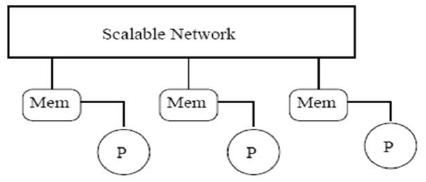
\includegraphics[width=8cm, height=4cm]{./eps/numa.jpg}
 \caption{a simple NUMA architecture design}
 \label{fig:numa}
\end{figurehere}

In Figure \ref{fig:numa} it's possible to see that in a NUMA multiprocessor the physical memory of the system is distributed among individual processors but is still globally addressable by all processors. Sometimes, it is preferable to have more than one processor in the same area. Each of this computational area containing memory block and CPU, whether it has one or more processors, is called node.Thus the cost of a memory access is dependent on where the memory unit addressed is located; relative to the processor some accesses may be local some may be remote. So, with the introduction of NUMA, data locality becomes an important factor because memory accesses have different costs depending on which memory unit is addressed. The scheduling module in the OS must cooperate with the memory management in order to let an application access data mostly from the local memory. NUMA systems can be classified in two categories, both for memory and for processor; regarding memory there are symmetrical and asymmetrical distribution, meaning that accessing different memory nodes can or cannot cost the same. Concerning processor it is possible to have homogeneous system, meaning that all processors are equal in speed and processing power, opposed to heterogeneous ones, where processors have different specifications even inside the same node. This type of architecture turns out to be exposed to some problems, and the most important are: cache coherence, scheduling and memory management.\par
\parindent 10mm In multiprocessor systems it is important to ensure cache coherency. If each processor has a cache that reflects the state of various parts of memory, it is possible that two or more caches may have copies of the same line. It is also possible that a given line may contain more than one lockable data item. If two threads make appropriately serialized changes to those data items, the result could be that both caches end up with different, incorrect versions of the line of memory. In other words, the system's state is no longer coherent because the system contains two different versions of what is supposed to be the content of a specific area of memory. There are 2 types of NUMA architectures that we have to analyse: NCC-NUMA (Non Cache Coherent) and CC-NUMA (Cache Coherent). In NCC-NUMA systems we have some software solutions, while in CC-NUMA we have a cooperation of both software and hardware solutions.\par 
\parindent 10mm Scheduling, memory management and thread migration are strictly connected.\\
In a multiprogrammed multiprocessor, the scheduler is not only responsible for deciding when to activate an application and when to suspend it, but is also responsible for determining how many processors to allocate to each application. In a scalable NUMA multiprocessor, it must further resolve the problem of which processors to allocate to which application since the memory reference times are not the same for all processor-memory pairs.\\
In NUMA systems, accesses to remote memory via interconnection are subject to various overheads. The bandwidth is lower than the bandwidth provided by the on-chip memory controller. The latency is higher as well: memory operations are processed by the local interface to the interconnect (arbitration may be needed if multiple cores access remote memory), a request is transmitted to another processor, and additional steps may be needed on this remote processor before the memory access can be done. Consequently, remote memory accesses suffer penalties of 1.5 to 2 times relative to local accesses. Good data locality is therefore highly desirable, i.e. the computations should take place on the processor that keeps their data. So memory management on these systems cannot be done without paying attention to process mapping, and a process scheduler that determines which processor executes a thread must consider where memory has been allocated.\\
With the introduction of NUMA systems, the scheduler now must also determine which processor(s) to allocate to which application. The relative positions of processors allocated to an application will affect the performance of it due to the difference in memory access times. Performance of an application may improve if all its allocated processors use only local memories \cite{Majo_memorysystem}.\\
Even among cache-coherent systems, these distributed architectures have non-constant physical distance between hardware components, causing their communication time to vary. Indeed, a core accesses local memory faster than other memory nodes. Most modern operating systems actually rely on a lazy allocation: when applications allocate virtual memory, the underlying physical pages are actually allocated upon the first access. While the primary advantage of this strategy is to decrease resource consumption, it brings an interesting feature usually referred to as first-touch: each page is allocated in the context of the thread that actually uses it first. The operating system is thus able to allocate physical pages on the memory node near the core that accesses it. However, if the first thread touching a page is not the one that will access it intensively in the future, the page may not be allocated "in the right place". For this reason, some applications manually touch pages during the initialization phase to ensure that they are allocated close to the threads that will actually access them.



%%%%%%%%%%%%%%%%%%%%%%%%%%%%%%%%%%%%%%%%%%%%%%%%%%%%%%%%%%%%%%%%%%%%%%%%%%%%%
\section{Solutions and Methods}

In this chapter will be presented some solutions about the problems introduced in previous section, divided by argument. Evaluations will be considered in the next chapter.

%-----------------------------------------------------------------------------
\subsection{Cache Coherence \\ Section}

As seen before, there are 2 types of NUMA architectures that will be analysed: NCC-NUMA (Non Cache Coherent - NUMA) and CC-NUMA (Cache Coherent - NUMA). \\
\subsubsection{Cache coherence in NCC-NUMA}
In NCC-NUMA systems, \emph{Kontothanassis and Scott} \cite{Kontothanassis94softwarecache} shown a new adaptive algorithm for software cache coherence that reduces interprocessor communication and scales to large numbers of processors; they then evaluate the tradeoffs among various write policies and the effect on performance of using remote memory access. Finally they also observe that certain simple program changes can greatly improve performance. this is done by following three steps. First, they maintain directory information for the coherence protocol in uncached shared locations, and access it with ordinary loads and stores, avoiding the need to interrupt remote processors in almost all circumstances. Second, while using virtual memory to maintain coherence at the granularity of pages, they never copy pages. Instead, they map them remotely and allow the hardware to fetch cache lines on demand. Third, while allowing multiple writers for concurrency, they avoid the need to keep old copies and compute diffs by using ordinary hardware write-through or write-back to the unique main-memory copy of each page. \par 
\parindent 10mm Concerning the same problem, \emph{Petersen and Li} \cite{Li95multiprocessorcache} presents a virtual memory based cache coherence that dinamically detects and resolves potential cache inconsistency using virtual memory techniques. VM-based cache coherence trades off design simplicity against incresed software overheads; this relies on that the existing memory transaction hardware on each processor that will be use to detect share accesses that could lead to memory incoherencies and special handlers execute the appropriate action to maintain cache coherence.
When a shared address space is created, the system initializes a page table for each processor. in this tables, the entries for a shared page will always have the same virtual-to-physical address tranlation. VM software will maintain the page tables at runtime according to a chosen memory consistency model. In the design of the VM-based algorithms synchronization variables are non cacheable to avoid the page fault overhead due to locks with high contention. Shared pages will therefore either contain ordinary data, and be cacheable, or synchronization variables, and be non-cacheable. Since most memory management units (MMUs) allow data to be cacheable on a per page basis, this property is used to mark pages that contain synchronization variables as non-cacheable.
By using off-the-shelf parts, state of the art components can be used in building multi-processors without additional design and fabrication efforts to incorporate cache coherence hardware.\\
Of this algorithm there are two implementation: VM-based Sequential Consistency (SC) and VM-based Release Consistency (RC).

\subsubsection{Cache coherence in CC-NUMA}
Regarding CC-Numa, \emph{Silvia Lametti} \cite{lametti} explains there are two protocols that are used to guarantee coherence: snooping and directory-based. Snooping system use a totally ordered network to directly broadcast coherence transactions to all processors and memory. Another solution is directory-based protocol; this one transmits coherence transactions over an arbitrary point-to-point network to the corresponding home directories which, in turn, redirect them to the processors caching the line. 

\begin{figurehere}
 \centering
 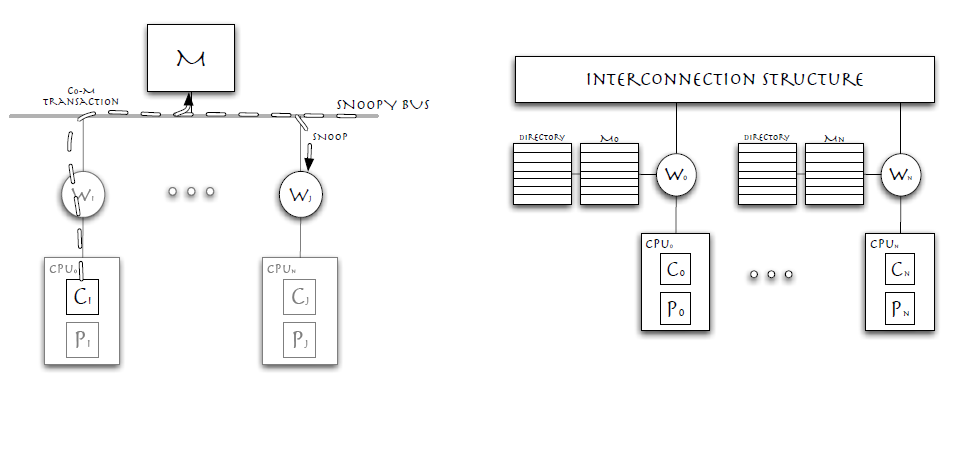
\includegraphics[width=8cm, height=4cm]{./eps/SnoopeDir.png}
 \caption{Snooping and Directory-based protocol}
 \label{fig:s&d}
\end{figurehere}

In all the systems which use the automatic techniques (snooping and directory), a proper protocol must exists in order to perform the required actions atomically. Two main techniques are used: \emph{invalidation}, \emph{update}.\\
Invalidation assumes that the only valid copy of a block is one of those, usually the last one, that has changed, invalidating all other copies (e.g. MSI and MESI in Figure \ref{fig:msimesi}); while update presumes that each modifcation of a cache block copy is communicated (multicasted) to all other caches (e.g. Dragon).\par
\parindent 10mm In the next chapter, invalidation and update techniques will be analysed only on directory-based protocol because it is clear from bibliography that large NUMA system does not support well BUS architecture due to large number of cores and, thus, messages that will limit the bandwith.

\begin{figurehere}
 \centering
 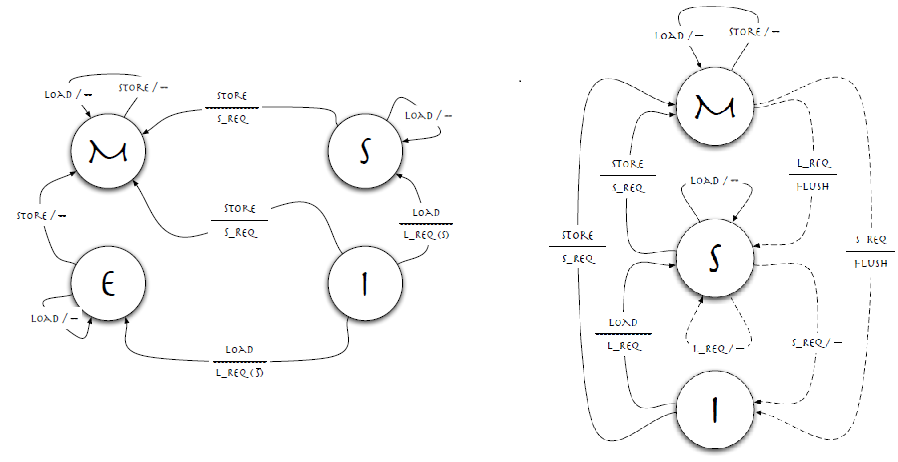
\includegraphics[width=8cm, height=4cm]{./eps/msimesi.png}
 \caption{MESI and MSI protocol}
 \label{fig:msimesi}
\end{figurehere}

%-----------------------------------------------------------------------------
\subsection{Scheduling and memory management \\ Section}
\emph{Chee-Shong Wu} \cite{Wu93processorscheduling} presents two tipe of policies: \emph{static} and \emph{dynamic}. \\
In the static policy, an application is allocated a fixed number of processors when it is activated, and it keeps these processors throughout its lifetime. Reallocations are performed only when some application completes. If there are no processors available, new arrivals are not started until some active application terminates and releases its set of processors. Applications hold the same number of processors from the beginning until the end of their execution without any readjustments.\\
In the dynamic policy, the number of processors allocated to an application may vary during its execution. The scheduler in this case has the responsibility of adjusting the number of processors allocated to an application according to its time varying parallelism, as well as to the system load. The hope is to avoid processor idling by quickly switching a processor from an application that does not require it to an application that can immediately utilize it.\\
\emph{Wu} presents a new static policy, called \emph{Immediate Start Static} (ISS). He implemented this policy because allocating an extra processor to an application that has sublinear speedup will cause some delay to all subsequent applications that use the same processors even though it may reduce the execution time of the application with the extra processor. Thus, it is important for a scheduler to be sensitive to the number of applications ready for execution and the overall system load. As the queue of ready applications becomes longer or as the system load increases, fewer processors should be allocated to each application in order to minimize overall average response time. A simple approach to making the scheduler sensitive to the length of the ready application queue and to the system load is to start a new application as soon as possible ideally immediately if there are active applications with more than one processor. This will likely require preempting processors from active applications at application arrivals. In the Immediate Start Static policy, when a new application arrives, if there are idle processors they are allocated to the new application; otherwise, the application is placed in a SSDF waiting queue. An active application that uses its last processor least effectively (the application with the smallest marginal loss of losing a processor) is identified and asked to give up a processor.
When a processor is given up by an active application due to the system scheduler's request, the processor is allocated to the first application in the waiting queue. At application completions, the actions are the same as in the static policy.\par
\parindent 10mm In \emph{Majo and Gross}'s paper \cite{Majo_memorymanagement}, is shown an hybrid solution between static and dynamic policies. They focus on the NUMA-Multicore-Aware Scheduling Scheme (N-MASS) that is an extension of the standart Linux scheduler. The reason why they need a new policy is that the performance of multiprogrammed workloads varies largely with the default Linux scheduler, and simple factors like the order in which workloads are started influence the performance readings. Because Linux scheduler balance only the CPU load and do not account for data locality or cache contention, processes might be mapped so that they use the memory system in the most ineffcient way possible. N-MASS, on the other hand, is a scheduling algorithm that takes into account memory system optimizations to quickly estimate the memory behavior of the scheduled programs on runtime (e.g NUMA penalty, that is the slow down of the same program executed remotely instead of locally). The N-MASS algorithm follows three steps. First, for each processor, it sorts the list of processes homed on the processor in descending order of the processes' NUMA penalty. Second, it maps the processes onto the system using the maximum-local policy. If the pressure on the memory system of the two-processor system is unbalanced, then in the third step the algorithm refines the mapping decision produced by the maximum-local mapping (as shown in Figure \ref{fig:n-mass_algo}).
This policy currently works on a NUMA with two processors but it can be extended to more cores.

\begin{figurehere}
 \centering
 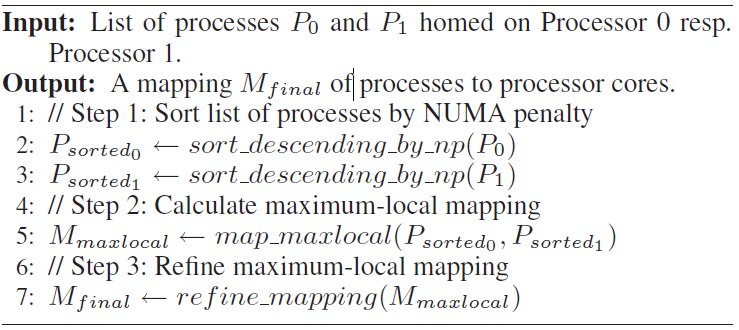
\includegraphics[width=8cm, height=4cm]{./eps/n-mass_algo.png}
 \caption{N-MASS: maps n processes onto a 2-processor NUMA-multicore system}
 \label{fig:n-mass_algo}
\end{figurehere}

The \emph{Li et al} 's paper \cite{Li07efficientoperating} presents AMPS, a scheduler that efficiently supports both SMP and NUMA-style performance-asymmetric architectures. AMPS contains three components: asymmetry-aware load balancing, fastercore-first scheduling, and NUMA-aware migration.\\
Asymmetry-aware load balancing ensures that the load on each core is proportional to its computing power. By defining a core's scaled computing power, P, to be its computing power divided by the system's minimum core computing power. At boot time, AMPS sets the scaled computing power of the core with the lowest frequency to one and any core with a F times higher frequency to F x S, where S is a less-than-one scaling factor. For any core with scaled computing power P, they define its scaled load, L, to be its run queue length divided by P. Let Lmax and Lmin be the maximum and minimum scaled load of a core in an asymmetric system. We define that the system is load-balanced if Lmax - Lmin is minor or equal then 1. In this asymmetric model, one unit of time on a core with P = x is equivalent to x units of time on a core with P = 1. Thus, by balancing threads proportionately to core computing power, AMPS facilitates fairness.\\
Faster-core-first scheduling (Figure \ref{fig:fcf}) enables threads to run on more powerful cores whenever they are under-utilized (i.e. L < 1), which load balancing alone cannot achieve in an asymmetric system. In AMPS threads move to and run on a faster core as long as the core is under-utilized. With this approach, a fast core of scaled computing power P behaves like P slow cores; in effect, they have transformed an asymmetric system into a symmetric one, which greatly simplifies the fairness support. For a newly created thread, they compute the new scaled load for each core assuming that the thread would run on it and choose the core with the minimum new scaled load to start the thread; if tied, they choose the faster core. AMPS does not allow a thread to migrate if the scaled load on the destination core after the migration can become greater than the  scaled load on the original core before the migration. This condition prevents a thread from migrating if its performance is not likely to improve.

\begin{figurehere}
 \centering
 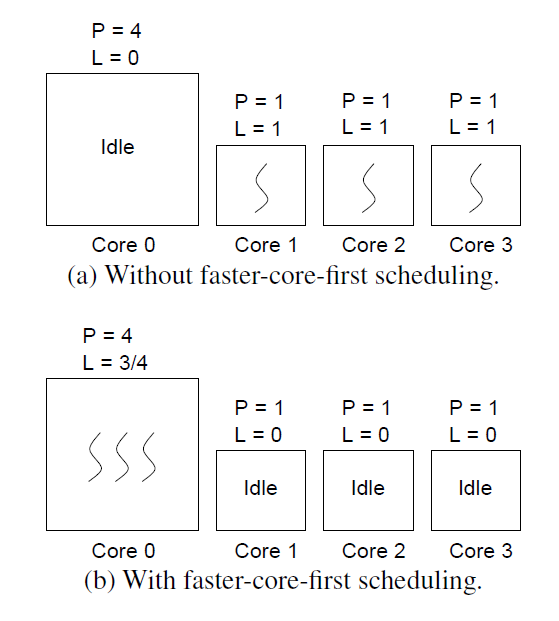
\includegraphics[width=8cm, height=9cm]{./eps/fcf.PNG}
 \caption{Example for Faster-core-first scheduling. \emph{P} denotes scaled computing power and \emph{L} denotes scaled load}
 \label{fig:fcf}
\end{figurehere}

NUMA-aware migration dynamically predicts thread migration overheads using memory resident sets and controls migration on NUMA-style architectures.
Qualitatively, a thread's migration overhead is high if the following conditions are both true, the thread incurs a high number of last-level cache misses after the migration and a large fraction of these Last Level Cache (LLC) misses require remote memory access.
When a thread T migrates from core A to core B, the algorithm predicts the migration overhead to be high if all of the following conditions are true:

\begin{itemize}
    \item Core A and core B are in different nodes.
    \item Core A is in a node for which thread T has the maximum Resident Set Size (the resident set of a thread on node N to be the set of pages that belong to the resident set of the thread and physically reside on node N - RSS)
   \item The RSS counter value of thread T for core A's node is greater than the LLC size of core B.
to the page.
\end{itemize}

If these conditions are true and thread T migrates, it will likely incur a large number of LLC misses and remote accesses to memory in core A's node.
Whenever there is a running thread to migrate, AMPS decides whether to allow the migration using one of the following policies:

\begin{itemize}
    \item \textbf{The Always policy:} with this policy, AMPS always allows a running thread to migrate regardless of the potential overhead.
    \item \textbf{The Same-Node policy:} with this policy, AMPS allows a running thread to migrate only within the same node and It is conservative in that it prevents a thread from migrating to a remote, faster core even when the actual migration overhead might be small.
   \item \textbf{The RSS policy:} this policy uses the resident-set-based prediction algorithm. It disallows a running thread to migrate if either it predicts the migration overhead to be high, or the thread is in the memory allocation phase.
to the page.
\end{itemize}

Recent research \cite{Balakrishnan05theimpact} advocates performance-asymmetric (or heterogeneous) architectures, where a processor contains multiple cores with the same instruction set but different performance characteristics (e.g., clock speed, issue width, in-order vs. out-of-order).\par
\parindent 10mm Finally, regarding thread migration, \emph{Hofmeyr and Colmenares} \cite{juggle} introduce a practical decentralized, user-space implementation of a proactive load balancer that emphasizes portability and usability that they called Juggle. They also analyze when it is conveninet to migrate a thread or not. Juggle executes periodically, every λ milliseconds (the load-balancing period) and attempts to balance an application that has \emph{n} threads running on \emph{m} processors, where \emph{n} is greater or equal then \emph{m}. The objective is to assign threads to processors such that the threads that have made the least progress now run on the processors with the lightest loads (the "fastest" processors). In practice, we classify threads as either ahead (above-average progress) or behind (below-average progress), and we classify processors as either fast or slow, according to whether they are less or more heavily loaded than average, respectively.  Juggle attempts to assign ahead threads toslow processors, and behind threads to fast processors.

%%%%%%%%%%%%%%%%%%%%%%%%%%%%%%%%%%%%%%%%%%%%%%%%%%%%%%%%%%%%%%%%%%%%%%%%%%%%%
\section{Evaluation}

In this section it will be discussed the difference between the proposed solutions above giving some value coming from direct confrontation.

%-----------------------------------------------------------------------------
\subsection{Cache coherence \\ Section}

\subsubsection{Cache coherence in NCC-NUMA}
Hardware coherence mechanisms for large-scalemachines are complex and costly, but existing software mechanisms for message-passing machines have not provided a performance-competitive solution. \par 
\parindent 10mm In  \emph{Petersen and Li} work \cite{Li95multiprocessorcache},  they present a comparative analysis of the performance achived by VM-based algorithm relative to \emph{no caching of shared data} (NO) and the \emph{MESI, invalidation-based, snoopy cache protocol} (Snoop). \\
As it is possible to observe from Figure \ref{fig:result1}, the NO, as expected, it has poor performance for most applications. It is possible to see that there can be a signicant performance gain from using VM-SC, rather than no-caching. However MUL performs best with no caching because only a little over 50% of all shared accesses hit in the cache. \par 
\parindent 10mm The best algorithm VM-based that they proposed is the RC version ( Figure \ref{fig:result1}). In fact the overhead due to coherency faults decreases in VM-RC because of the relaxed memory consistency restrictions, and accounts for most of the improvement of each application. They then compared RC with Snoop; the execution time breakdown for each application shows two reasons for the difference in performance between VM-RC and Snoop: the overhead due to the VM-based implementation of RC, the time a processor stalls on a full write-buffer, and the time a processors spends waiting for memory loads to complete. The cache miss ratio under Snoop and VM-RC is very similar for all applications, therefore the number of memory accesses due to shared and private accesses that require a bus transaction is very close. The total memory access time in VM-RC is affected mostly by memory  accesses issued by the algorithm and due to write-throughs. Relaxing the memory consistency models, and hence synchronizing the processors in the system only  when the application requires to do so, allows the VM-based RC cache coherence scheme to perform very well. 


\begin{figurehere}
 \centering
 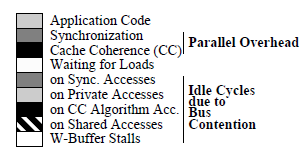
\includegraphics[width=6cm, height=3cm]{./eps/Legenda_VM-based.PNG}
 \caption{Legend of next column diagram}
 \label{fig:legend}
\end{figurehere}

\begin{figure*}
 \centering
 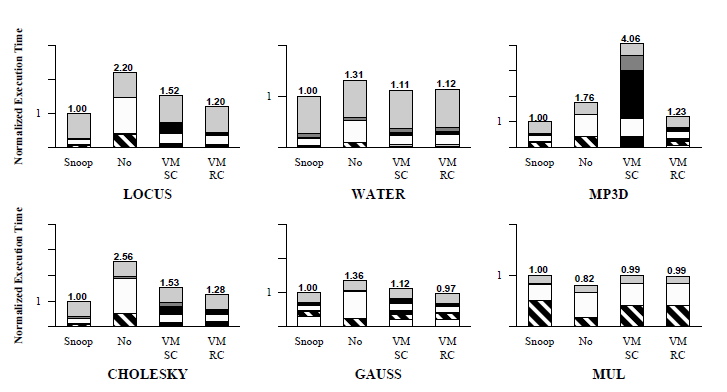
\includegraphics[width=14cm, height=7cm]{./eps/result1.PNG}
 \caption{Performance of VM-based schemes}
 \label{fig:result1}
\end{figure*}

\parindent 10mm In their articles,\emph{ Kontothanassis and Scott} \cite{Kontothanassis94softwarecache} used virtual memory protection bits to enforce consistency at the granularity of pages allowing more than one processor to write a page concurrently,and used a variant of release consistency to limit coherence operations to synchronization points.\\
As in the work of \emph{Petersen and Li} \cite{Li95multiprocessorcache}, they exploit the global physical address space to move data at the granularity of cache lines: instead of copying pages, thay  map them remotely, and allow the hardware to fetch cache lines on demand. The protocol employs a distributed, non-replicated directory data structure that maintains cacheability and sharing information, similar to the coherent map data structure. A page can be in one of the following four states:
\begin{itemize}
    \item \textbf{Uncached}, no processor has a mapping to the page. This
is the initial state for all pages.
    \item \textbf{Shared}, one or more processors have read-only mappings
to the page.
   \item \textbf{Dirty}, a single processor has both read and write mappings
to the page.
   \item \textbf{Weak},  two or more processors have mappings to the page
and at least one has both read and write mappings.
\end{itemize}

They, then, compared their software protocol to the protocol devised by \emph{Petersen and Li} \cite{Li95multiprocessorcache}. They found out that their implementation was significantly better then the other and even on applications that in programs where coherence is less important, their protocols still provide reasonable performance improvements over the remaining ones, ranging from 2\% to 35\%.

\begin{figurehere}
 \centering
 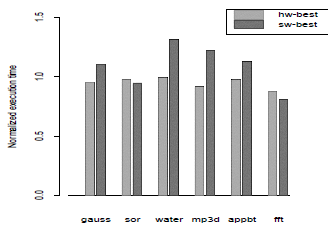
\includegraphics[width=7.5cm, height=6cm]{./eps/result16proc.png}
 \caption{comparative software and hardware system performance on 16 processors}
 \label{fig:16proc}
\end{figurehere}


\begin{figurehere}
 \centering
 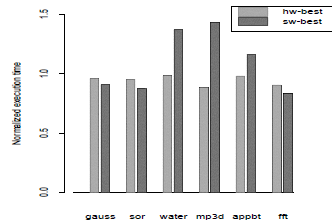
\includegraphics[width=7.5cm, height=6cm]{./eps/result64proc.png}
 \caption{comparative software and hardware system performance on 64 processors}
 \label{fig:64proc}
\end{figurehere}

Int the end, however, they compared their software solutions to hardware existing solutions and find out that in all cases the performance of the software protocol is within 55\% of the hardware protocol as shown in Figure \ref{fig:16proc} and in Figure \ref{fig:64proc}.\par
\parindent 10mm Thus, in the following section will be shown a couple of hardware solutions tipically found on cc-NUMA.

\subsubsection{Cache coherence in CC-NUMA}
As previously said, CC-NUMA have hardware solutions to manage coherency and there exists two different implementation depending on the architecture: BUS or an interconnection structure. According to the implemented architecture, a different solution is used to update and control caches: snooping and directory-based. It is important to choose a good protocol for cache coherence on a cache coherent system, thus write invalidate and write update have been examined to choose the best.\par
\parindent 10mm Update protocol conserves bandwidth and needs only one update  transaction to keep multiple sharers up to date but generates a lot of unnecessary traffic when a single processor writes  repeatedly to a block and no other processor accesses the block. On the other hand, invalidate does exactly the opposite and this means that there is not a best solution because both depend on the kind of application running.\par
\parindent 10mm As previously said, there are two hardware architecture: with a bus or with an interconnection structure. Nowadays it is common knowledge that using a bus architecture with a large number of nodes doesn't work very well because this solution presents some problems due to the fact that every request is broadcasted on the BUS and this tends to overfill the bandwidth. Even an interconnection structure has some problems, typically the overhead of directory indirection and message sequencing, but it is a fair price to pay compared to the benefits.\cite{moh}\par
\parindent 10mm In \emph{Majo and Gross} work, they show that in some cases, when the machine is highly loaded, the cross-chip interconnect outperforms the on-chip memory controller. Mapping computations so that all memory traffic flows through the local memory interface is bound to be suboptimal in many situations. \cite{Majo_memorysystem}

%-----------------------------------------------------------------------------
\subsection{Scheduling and memory management \\ Section}

Regarding static and dynamic polices \emph{Wu} believes that by utilizing application characteristics, it is possible for a static policy to outperform a dynamic policy in NUMA systems; therefore he preents a comparison between the two policies as shown in Figure \ref{fig:tabella}.


\begin{figurehere}
 \centering
 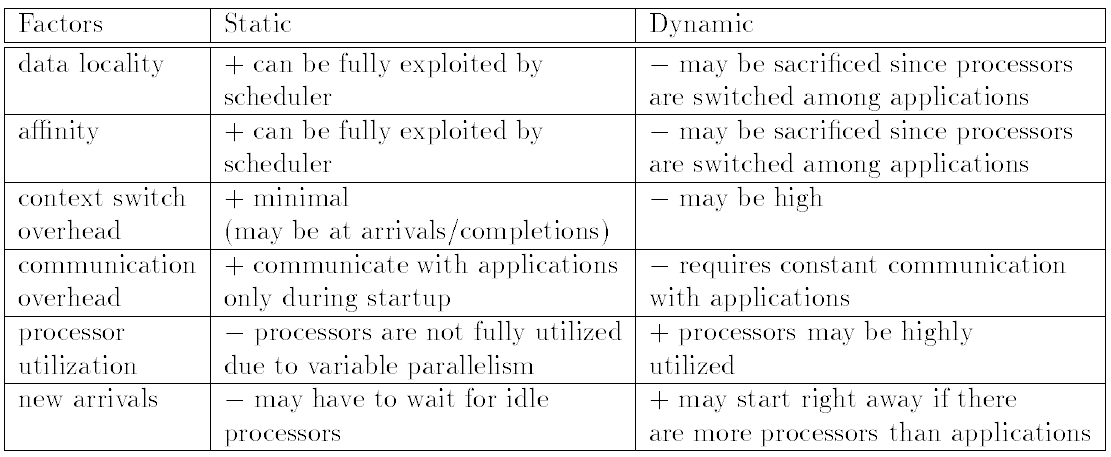
\includegraphics[width=8cm, height=4cm]{./eps/tabella.png}
 \caption{Comparison of performance factors of static and dynamic policies}
 \label{fig:tabella}
\end{figurehere}

In order to prove his theory he compares ISS policie with the existing ones (static and dynamic).\\
The first comparison is versus static (STA) and he argues that one of the drawbacks of the Static policy is that it fails to start an application soon after it has arrived. The Immediate Start Static policy, however, addresses this drawback and starts a newly arrived application almost immediately. To determine the effect of this change in the static policy, and the benefit of reallocating both at arrivals and completions, the performance of STA and ISS were studied and compared.
Figure \ref{fig:issvssta} presents the performance of STA and ISS on 12  processors. Workload represents the minimum average response time without multiprogramming. Notice that this minimum average response time is 7.2\% larger for the ISS policy than for the STA policy because the implementation of ISS is slightly more complicated than STA.

\begin{figurehere}
 \centering
 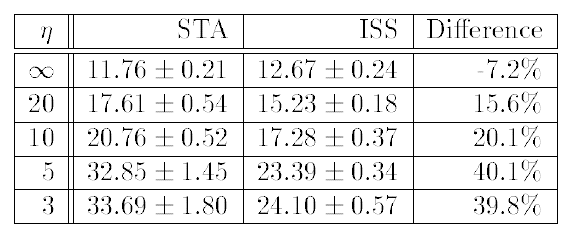
\includegraphics[width=8cm, height=3cm]{./eps/issvssta.png}
 \caption{Mean response time under STA and ISS}
 \label{fig:issvssta}
\end{figurehere}

In all four workloads studied, ISS outperforms STA by  15-40\%. The STA policy prevents the completion of small applications by not starting a new application soon after it arrives, even though there may be other applications with more than one processor. This delay in completion of one application will lead to further delay to subsequent applications in the workload. As a result, the mean response time of STA is much worse than ISS. The benefit of immediately starting a new application becomes more apparent as the system load increases. The longer the waiting queue, the poorer the performance is since remaining applications in the workload are subject to more subsequent delays. Since STA is a policy that reallocates only at completions, and ISS is a policy that reallocates both at arrivals and completions, the result of this experiment also indicates the importance of reallocating at both arrivals and completions.\\

The second comparison is versus dynamic (DYN) policy. The slightly worse performance of DYN compared to ISS is because of the extra overhead in DYN. These overheads include the overhead of context switching among applications, the overhead of constant communication between the scheduler and applications, the overhead of more frequent cache reloads, and the overhead of more costly memory accesses due to loss of data locality. The performance of the Immediate Start Static policy compared to the Dynamic policy is presented in the following Figure \ref{fig:issvsdyn}.

\begin{figurehere}
 \centering
 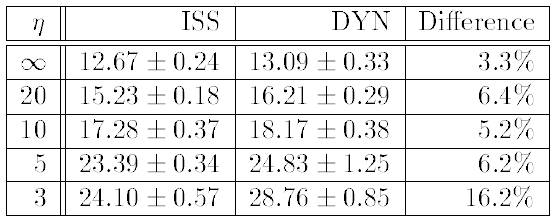
\includegraphics[width=8cm, height=3cm]{./eps/issvsdyn.png}
 \caption{Mean response time under STA and DYN}
 \label{fig:issvsdyn}
\end{figurehere}

As the service demands of applications become larger, the DYN policy becomes more appropriate. When the overhead of DYN is made smaller relative to the service demands of applications, the cost of frequent reallocating processors in DYN can be justified; this is also the result found within Juggle \cite{juggle}, where it is said that their parameter must be at minumum the overhead of Juggle itself (about \emph{100 microseconds}); when the parameter is on the order of the scale at which the OS scheduler operates, the assumption that each thread gets a fair share of a processing element breaks down. We can see this in Figure \ref{fig:juggle}, which shows how performance degrades as the parameter falls below \emph{10ms}, which is the scheduling interval on that particular system. As the parameter reduces even further, the \emph{100 microseconds} overhead starts to impact performance.

\begin{figurehere}
 \centering
 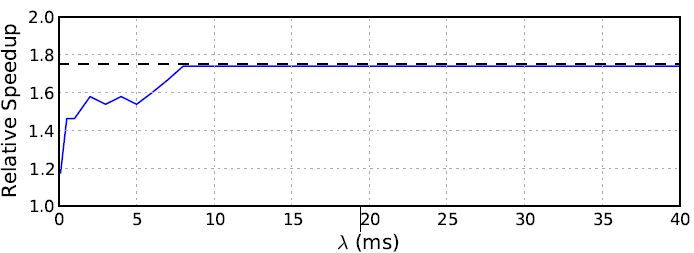
\includegraphics[width=8cm, height=3.5cm]{./eps/juggle.png}
 \caption{Effect of decreasing parameter.}
 \label{fig:juggle}
\end{figurehere}

However, dynamic scheduler might be inappropriate in NUMA systems; the simpler and more static approach of the ISS policy attempts to maintain data locality and cache affinity by avoiding frequent reallocations of processors, at the same time reducing overhead. When remote access times are made larger (as they would be in a larger system), the ISS policy continues to dominate the DYN policy for a mixed workload. As a result, ISS performs better than the more dynamic policy, DYN.

The importance of data locality is also shown in \emph{Majo and Gross} 's paper \cite{Majo_memorymanagement}. They present two cases: when memory allocation in a NUMA-multicore system is balanced (the cumulative memory demand of processes homed on each processor in the system is approximately the same), then it is beneficial to simply map processes onto the architecture so that data locality is favored, and avoiding cache contention does not bring any benefits; otherwise, when the memory allocation in the system is unbalanced (the sum of the memory demands of processes homed on each processor in the system is different), then mapping processes so that data locality is maximized can lead to severe cache contention; in these cases refining the maximum-local mapping so that cache contention is reduced improves performance, even with the cost of some processes executing remotely. N-MASS algorithm, an extension of the maximum-local, was created to solve the problem with unbalanced memory allocation.



\section{Conclusion}
We want to discuss and recap about the results reached by our references, proposing an our personally opinion concerning the NUMA architecture issues.
Cache coherence is an important issue in multiprocessor systems and we have seen different solutions, both software and hardware. It is our opinion that nowadays the best solution is an hardware solution with an interconnection structure on most NUMA.

Software solutions, even if are not as performing as hardware ones, remain a less expensive solution good enough for NUMA with a small number of nodes and with low request performance and are, instead, really good for NUMA with many nodes and BUS architecture.

Probably some hybrid solution, like using a bus within processors on the same node and an interconnected structure to connect different nodes or even a mixture of both hardware and software solution within the same system, could lead to good results and should be investigate.
However the best thing to seek now is a way to know which resources a program will access and if this is done a lot of times or not, leading to the best choice of the protocol to be used, update or invalidate, bestowing a good speed up of performances.

% We suggest the use of JabRef for editing your bibliography file (Report.bib)
\bibliographystyle{splncs}
\bibliography{Report}

\end{multicols}
\end{document}
